\documentclass{jsarticle}
\usepackage{here}
\usepackage[dvipdfmx]{graphicx}

\begin{document}


\title{計数工学プログラミング演習最終レポート}
\author{計数工学科システム情報学コース3年\\03-190615\\工藤龍}
\maketitle

\section{課題内容}

疎行列の2乗を様々な手法で計算し,実行時間を測定した.


\section{手法}

今回の実験に用いたのは,以下の三つのアルゴリズムである.
\begin{itemize}
\item 密行列
\item 疎行列(三重ループ)
\item 疎行列(リスト)
\end{itemize}


\section{実験結果}

\begin{figure}[H]
  \begin{center}
  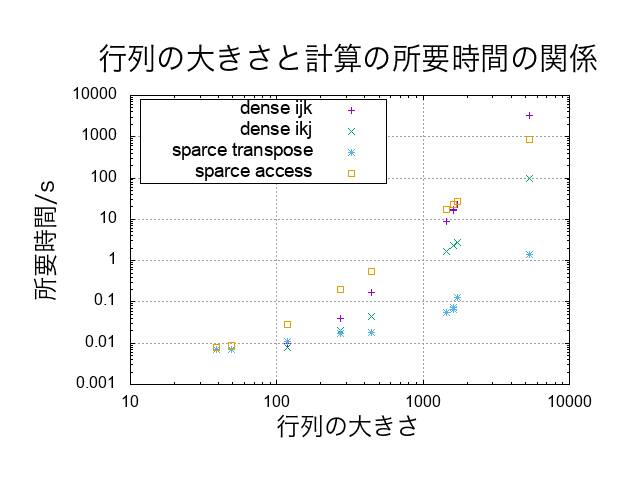
\includegraphics[width=10cm]{../graph.png}
  \end{center}
\end{figure}


\section{考察}

解説文を読んで,このソースをいろいろと変更してみましょう。

\end{document}
